% **************************************************
% TESIS: Título de la tesis doctoral
% EDITOR: Jesús Guadalupe P. Flores
% LUGAR Y FECHA: Mineral de la Reforma, Hidalgo, México. 2021.
% **************************************************

% **************************************************
% Definición de documento:
% **************************************************
\documentclass{book}
\usepackage{LauraGC}

% **************************************************
% Cargar y configurar el paquete BibLaTeX:
% **************************************************
\usepackage[
	natbib = true,
	backend = biber,
	style = authoryear-comp,
	citetracker = true,
	maxcitenames = 1,
	bibstyle  = apa,
	uniquename = false,
	refsection = chapter,
	sortcites = true,
	sorting   = ynt
	]{biblatex}

\DeclareLanguageMapping{spanish}{spanish-apa}


% **************************************************
% Usar la compresión, excepto la primera vez:
% **************************************************
\AtEveryCitekey{\maxminformat} % Citar todos los autores
\def\fls{\setcounter{maxnames}{6}\clearfield{namehash}} %Primera vez que se van a citar menor a 6 autores
\def\nfgt{\setcounter{minnames}{1}\setcounter{maxnames}{1}} %no primera vez y mayor a 2 autores
\def\flt{\setcounter{maxnames}{\value{labelname}}} %primera vez y menor que 2 autores

\def\maxminformat{%
	\ifnumgreater{\value{labelname}}{2} %Si el número mayor de autores fuera 2
	{\ifciteseen
	{\nfgt}
	{\fls}}
    {\flt}}


% **************************************************
% Add a comma and replace "and" with "&" before last coauthor:
% **************************************************
\DeclareDelimFormat{finalnamedelim}
	{\ifnum\value{liststop}>2 \finalandcomma\fi\addspace\&\space}


% **************************************************
% Comma before ampersand in last author bibliography apa-biblatex
% **************************************************  
\DefineBibliographyExtras{spanish}{\def\finalandcomma{\addcomma}}

\DeclareDelimFormat[bib,biblist]{finalnamedelim}{%
  \ifthenelse{\value{listcount}>\maxprtauth}
    {}
    {\addcomma\space\&\space}}


% **************************************************
% Reemplazar el "y col." por et al.:
% **************************************************	
\DefineBibliographyStrings{spanish}{%
    andothers = {\it et\addabbrvspace al\adddot}
}


% **************************************************
%Cargamos los ficheros con las referencias:
% **************************************************	

% Referencias del CAPÍTULO 1:
\addbibresource{main/RefChap1.bib}

% Referencias del CAPÍTULO 2:
\addbibresource{main/RefChap2.bib}

% Referencias del CAPÍTULO 3:
\addbibresource{main/RefChap3.bib}

% **************************************************
%	Configuración del idioma:
% **************************************************
\usepackage[utf8]{inputenc}
\usepackage[english, spanish, es-tabla]{babel}
\selectlanguage{spanish}


% **************************************************
%	Paquetes:
% **************************************************
\usepackage{lipsum} % Incluir texto en latín de relleno
\usepackage{subfiles} %incluir tablas a manera de sub-archivos
\usepackage[version=4]{mhchem} %escribir símbolos químicos en el texto
\usepackage{chemfig} %estructuras químicas
\usepackage{amsmath,amsthm,amsfonts,amssymb,gensymb,textcomp}
\usepackage{fourier-orns}
\usepackage{graphicx} % Insertar figuras
\usepackage{subfig} % Insertar subfiguras
\usepackage{lscape} %no rotation of the page 
\usepackage{listings}
\usepackage{tikz}
\usepackage[final]{pdfpages} %Configuración de PDF Externos
\usepackage{makeidx} % Índice alfabético
\usepackage[printonlyused,withpage]{acronym} % Crear lista de acrónimos.
\usepackage{comment} %Insertar entornos de comentarios
\usepackage{enumitem} %Enlistar con números romanos
\usepackage[numbib]{tocbibind} %Agrega índices referencias y tablas de contenidos
\spanishdecimal{.} %Cambia las comas por puntos en los números


% **************************************************
%	Configuración de secciones:
% **************************************************
\usepackage{titlesec}
\setcounter{secnumdepth}{3} %enumerar sub-subsecciones
%\setcounter{tocdepth}{3}  %para que las sub-subsecciones aparezcan en el índice


% **************************************************
%	Formato de hipervínculos y datos del editor:
% **************************************************
\usepackage{hyperref}
\hypersetup{
	colorlinks=true,
	citecolor=iColor003,
	filecolor=iColor003,
	linkcolor=iColor003,
	urlcolor=iColor003,
	bookmarksopen=true,
	pdfpagelayout=TwoPageRight,
	pdftitle={Título de la tesis},
	pdfauthor={Jesús Guadalupe Pérez Flores},
	pdfsubject={Tesis doctoral},
	pdfproducer={LaTeX},
	pdfkeywords={Palabras, clave, de, la, tesis}
}


% **************************************************
%	Ajustar longitud de la barra sobre la X:
% **************************************************
\makeatletter
\newcommand*{\Xbar}{}%
\DeclareRobustCommand*{\Xbar}{%
  \mathpalette\@Xbar{}%
}
\newcommand*{\@Xbar}[2]{%
  \sbox0{$#1\mathrm{x}\m@th$}%
  \sbox2{$#1x\m@th$}%
  \rlap{%
    \hbox to\wd2{%
      \hfill
      $\overline{%
        \vrule width 0pt height\ht0 %
        \kern\wd0 %
      }$%
    }%
  }%
  \copy2 %
}
\makeatother


\graphicspath{{pictures/}} % Localizacion de las figuras

	\makeindex % Crear índice


\begin{document}
% **************************************************
% Comienza la escritura del documento:
% **************************************************
	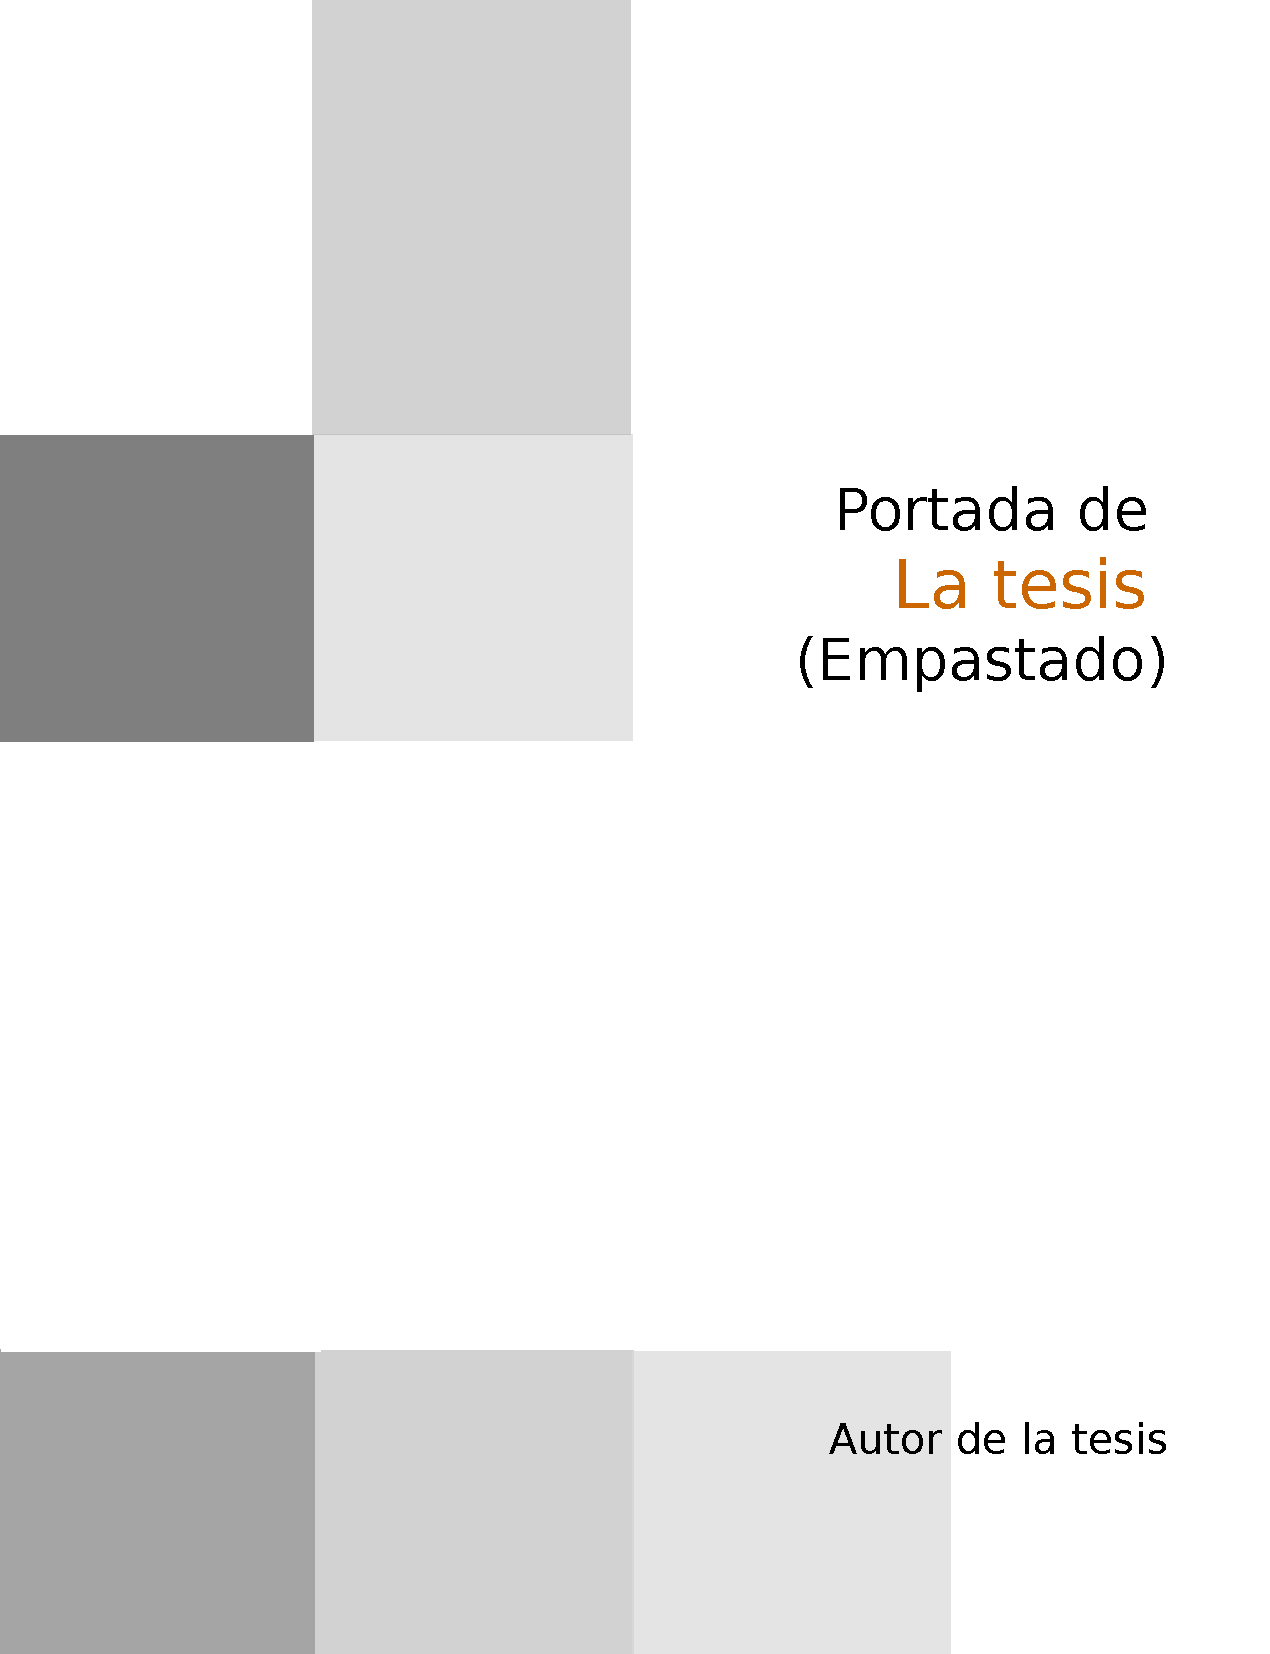
\includepdf[pages=1-2]{front/PORTADA}
	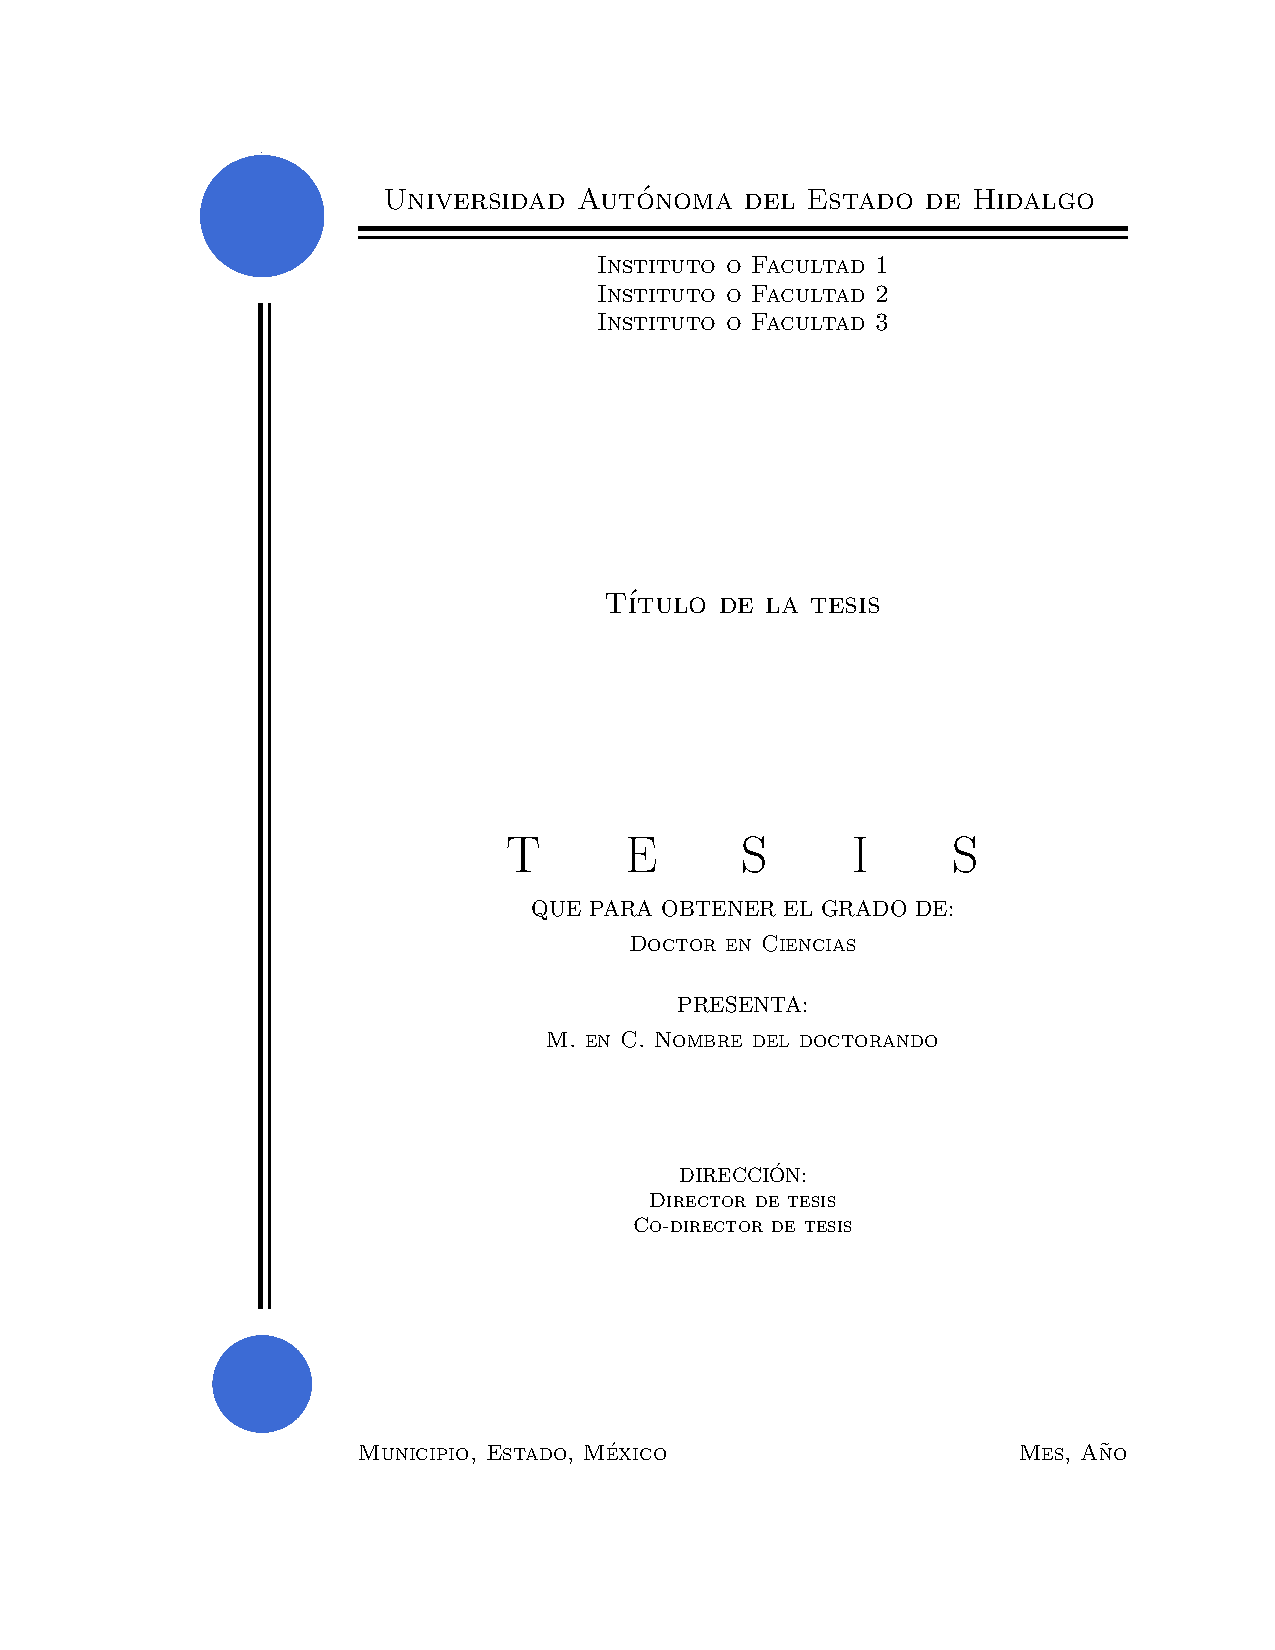
\includepdf[pages=1-2]{front/PortadaTesis} %[pages=inicial-final]{nombre_del_documento}
	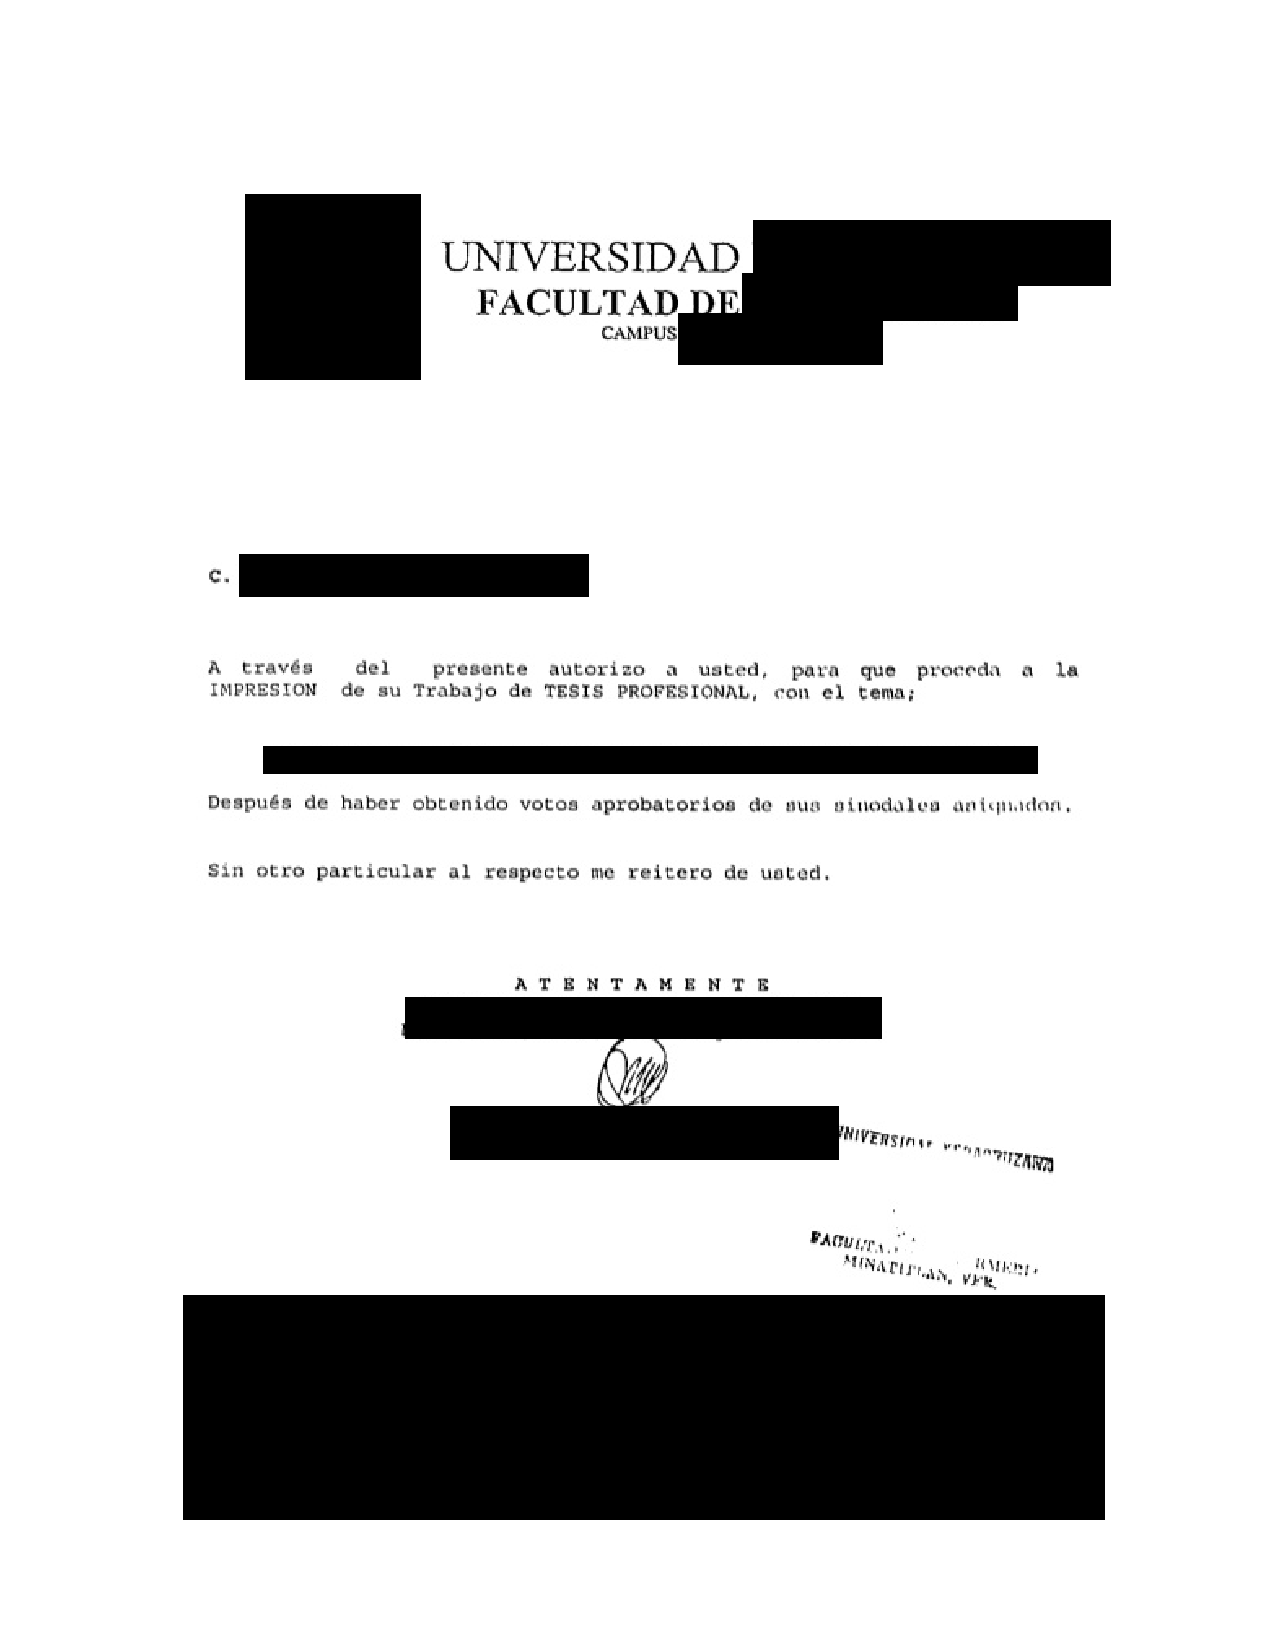
\includepdf[pages=1-2]{front/AutorizacionDeImpresion}
	%\begingroup
\clearpage
\begin{changemargin}{2cm}{2cm} 

    \thispagestyle{empty}
    \vspace*{\fill}
    
%    \dedicatoriafont

\begin{center}
    Dedico esta \textsc{Tesis}:
\end{center}

\begin{center}
    A~\textsc{mi madre}\ldots
\end{center}

\begin{center}
    A~\textsc{mi hermana}\ldots
\end{center}

\begin{center}
    A~\textsc{Laura García Curiel}, eres liberosis en un mundo que en general es bastante hostil, pero que vale la pena vivirlo. Eres paz y sosiego en medio de la guerra, y eres primavera a la mitad del invierno. Gracias por amarme, por impulsarme y por creer en mí\ldots
\end{center}
  
\begin{center}
    \textsc{A todos} los que no respetan los esquemas preestablecidos, a los soñadores, a los locos, a los raros y a los incomprendidos, a los inclaudicables, a los que no encajan, a los entusiastas, a los idealistas, a los emprendedores y a los visionarios del mundo. Porque los cambios más importantes para la humanidad, los grandes avances y los grandes descubrimientos los hacen \textsc{ustedes}\ldots
\end{center}
    
\begin{center}
	\usefont{T1}{LobsterTwo-LF}{bx}{it}
	Jesús Guadalupe Pérez Flores
\end{center}

\begin{center}
	\Huge
	\textxswup
\end{center}

    \vspace*{\fill}

\end{changemargin}
\clearpage
%\endgroup
 % Dedicatoria
	\begingroup
\pagestyle{empty} % Remueve los números de página

\chapter*{Agradecimientos}

\textsc{A mi paciencia}\ldots


\thispagestyle{empty}
\cleardoublepage
\endgroup % Agradecimientos

% **************************************************
\frontmatter %InicioDocumento
% **************************************************
	\tableofcontents %Índice general
	\listoffigures %Índice de Figuras
	\listoftables %Índice de Tablas

	% **************************************************
\chapter*{Lista de acrónimos}
\addcontentsline{toc}{chapter}{Lista de acrónimos}
\markboth{LISTA DE ACRÓNIMOS}{LISTA DE ACRÓNIMOS}
% **************************************************

\begin{acronym}[TDMA] 
% ------------- Inicia Lista -----------------------
\acro{AX}{arabinoxilanos}
\acro{aLAraf}[$\alpha$-{\scriptsize L}-{A}ra\textit{f}]{$\alpha$-{\scriptsize L}-arabinofuranosil}
\acro{BDXylp}[$\beta$-{\scriptsize D}-{X}yl\textit{p}]{$\beta$-{\scriptsize D}-xilopiranosil}
% ------------- Termina Lista -----------------------
\end{acronym}

 % Lista de acrónimos
	% **************************************************
\chapter*{Abstract}
\addcontentsline{toc}{chapter}{Abstract} % Agregar al índice
\markboth{ABSTRACT}{ABSTRACT} % Encabezado 
% **************************************************

\lettrine[lines=3]{B}{rewers'} spent grain (BSG) is the most abundant by-product generated from the beer-brewing process and constitutes a potential source for arabinoxylans (AX) extraction. \lipsum[6]
 % Abstract
	% **************************************************
\chapter*{Resumen}
\addcontentsline{toc}{chapter}{Resumen} % Agregar al índice
\markboth{RESUMEN}{RESUMEN} % Encabezado 
% **************************************************

\lettrine[lines=3]{E}{l bagazo} de cebada (BSG) es el principal subproducto generado durante el proceso de elaboración de la cerveza y constituye una fuente potencial para la extracción de arabinoxilanos (AX). \lipsum[6]. % Resumen

% **************************************************
\mainmatter %ContenidoPrincipal
% **************************************************

	% **************************************************
\chapter{Título del capítulo 1: Versión laraga del título}
\chaptermark{Versión corta del título}
% **************************************************
\chapterquote{Escribe una frase aquí para iniciar el \textsc{Capítulo 1}\ldots}{Autor de la frase}{Datos adicionales aquí, \oldstylenums{2004}}
% **************************************************


% Resumen:
\begin{ResumenPhDThesis}
\begin{changemargin}{1cm}{1cm}
\lettrine[lines=3]{E}{scribir aquí} el resumen del \textsc{Capítulo 1}: \lipsum[3]
\end{changemargin}
\end{ResumenPhDThesis}


% **************************************************
\section{Introducción}
\index{xilanos}
% **************************************************
El capítulo 1 se trata de los antecedentes generales de la investigación, puede ser una revisión. Escribir en este apartado, una introducción del \textsc{Capítulo 1}: \lipsum[3]


% **************************************************
\section{Uso de acrónimos}
% **************************************************
Aquí se presenta un ejemplo del uso de acrónimos: Los \acf{AX} poseen una cadena principal de \acf{BDXylp} unidos mediante enlaces $\beta$-(1$\rightarrow$4), a los que se unen grupos de  \acf{aLAraf} que están unidos mediante enlaces $\alpha$-(1$\rightarrow$3) y/o $\alpha$-(1$\rightarrow$2) \citep{perez2019physicochemical}. 

\lipsum[2]


% **************************************************
\section{Fórmulas químicas}
% **************************************************
En este documento tambien se puede hacer uso de símbolos y fórmulas químicas gracias al paquete \textbf{mhchem}, de la siguiente manera: se ha realizado extracción de AX con \ce{NaOH}, \ce{KOH}, \ce{Ba(OH)2} y \ce{Ca(OH)2}. De igual manera, se han utilizado diferentes combinaciones de medio básico con \ce{H2O2}, \ce{NaBH4}, \ce{Na2SO3}, \ce{Na2S2O4} y \ce{NaClO2}.

Iones: \ce{Pb^2+}, \ce{Ca^2+}.

Enlaces: \ce{C-H}.

Sales: \ce{CaCl2.H2O}, \ce{FeCl2.4H2O}, \ce{K2CO3}, \ce{(NH4)2S2O8} y \ce{FeCl3.6H2O}.

Radicales hidroxilo: \lewis{4.,OH}.

Otros: $\beta$-{\scriptsize D}-{X}yl\textit{p}.



% **************************************************
\section{Citas}
% **************************************************
\subsection{Varios papers en el mismo año}
% **************************************************
En esta tesis se utilizó Bib{\LaTeX} para citar en formato APA, sexta edición. Se pueden comprimir las citas cuando hay varias publicaciones del mismo autor en el mismo año: \citep{king200nonstationary, king2000semiparametric, king2001gaussian,king2001regression}.

Primera vez: \citep{wang2012optimization}.

Segunda vez: \citep{wang2012optimization}.

Primera vez: \citep{wang2014optimisation}.

Segunda vez: \citep{wang2014optimisation}.

Juntos: \citep{wang2014optimisation, wang2012optimization}.


% **************************************************
\subsection{Varios casos}
% **************************************************
Menos de 6 autores por primera vez: \citep{rosicka2016influence}.

Menos de 6 autores por segunda vez: \citep{rosicka2016influence}

Más de 6 autores por primera vez: \citep{perez2019physicochemical}.

Más de 6 autores en el mismo año: \citep{bender2017optimization,bender2017chemical}.

Varios autores en orden cronológico: \citep{zhang2014extraction, gonzalez2015covalently, rosicka2016influence}.

Sólo 2 autores por primera vez: \citep{kamboj2014physicochemical}.

Sólo 2 autores por segunda vez: \citep{kamboj2014physicochemical}.



% **************************************************
\section{Conclusiones}
% **************************************************
Escribir las conclusiones del \textsc{Capítulo 1}: \lipsum[2]


% **************************************************
% Referencias
% **************************************************	
\begin{refcontext}[sorting=nyt]
\printbibliography[title={Referencias}, heading=subbibintoc]
\end{refcontext}
 %Capítulo 1
	% **************************************************
\chapter{Título del capítulo 2: Versión laraga del título}
\chaptermark{Versión corta del título}
% **************************************************
\chapterquote{Escribe una frase aquí para iniciar el \textsc{Capítulo 2}\ldots}{Autor de la frase}{Datos adicionales aquí, \oldstylenums{2009}}
% **************************************************

% Resumen:
\begin{ResumenPhDThesis}
\begin{changemargin}{1cm}{1cm}
\lettrine[lines=3]{E}{scribir aquí} el resumen del \textsc{Capítulo 2}: \lipsum[3]
\end{changemargin}
\end{ResumenPhDThesis}



% **************************************************
\section{Introducción}
% **************************************************
Escribir en este apartado, una introducción del \textsc{Capítulo 2}: \lipsum[1]

Uso de listas con números romanos: 

\begin{enumerate}[label=\roman*.]
	\item Paso uno;
	\item Paso dos;
	\item Paso tres;
	\item Paso cuatro;
	\item Paso cinco.
\end{enumerate}


% **************************************************
\section{Escribe el nombre de la sección del capítulo}
\index{niveles!sección del capítulo}
% **************************************************
\lipsum[2]

% **************************************************
\subsection{Escribe el nombre de la subsección}
\index{niveles!subsección del capítulo}
% **************************************************
\lipsum[2]

% **************************************************
\subsubsection{Escribe el nombre de la subsubsección}
\index{niveles!subsubsección del capítulo}
% **************************************************
\lipsum[2]

% **************************************************
\paragraph{Escribe un párrafo} % Esto es en vez de una sub-sub-subsección 
\index{niveles!párrafo}
% **************************************************
\lipsum[2]



% **************************************************
\section{Figuras}
% **************************************************
\subsection{Una figura}
\index{insertar!figura}
% **************************************************
A continuación se presenta el ejemplo de cómo insertar la Figura~\ref{fig:EjemploFigura}:

\begin{figure}[htp]
	\centering
	
\includegraphics[width=1\linewidth]{FiguraX.png}
    \caption[Título de una figura.]% Así es como aparece en el índice de figuras
    {Título de una figura con una descripción más detallada. \lipsum[1]} % Se puede redactar una descripción con más detalles
    \label{fig:EjemploFigura}
\end{figure}


% **************************************************
\subsection{Una figura con rotación}
\index{insertar!figura con rotación}
% **************************************************

En la Figura~\ref{fig:FiguraRotacion} se muestra una figura con rotación:

%Insertar una figura con rotación
\begin{sidewaysfigure}[htp]
	\centering 
	
\includegraphics[width=1\linewidth]{FiguraX.png}
    \caption[Título de una figura con rotación.]% Título que aparece en el índice de figuras
    {Título de una figura con rotación con una descripción más detallada. \lipsum[1]} % Descripción más larga de la figura
    \label{fig:FiguraRotacion}
\end{sidewaysfigure}


% **************************************************
\subsection{Subfigura}
\index{insertar!subfiguras}
% **************************************************
En la Figura~\ref{Fig:SubfigurasEjemplo} se incluyen subfiguras, es decir: La Figura~\ref{Fig:SubFig1} y la Figura~\ref{Fig:SubFig2}. 


\begin{figure}[htp]
   \centering
   %%---- Primera subfigura ----
   \subfloat[Título de la subfigura 1]{ %Es opcional
        \label{Fig:SubFig1}         %% Etiqueta para la primera subfigura
        
\includegraphics[width=0.455\textwidth]{FiguraX.png}}
   \hspace{0.05\linewidth}
   %%---- Segunda subfigura ----
   \subfloat[Título de la subfigura 2]{ %Es opcional
        \label{Fig:SubFig2}         %% Etiqueta para la segunda subfigura
        
\includegraphics[width=0.455\textwidth]{FiguraX.png}}
   \caption[Título de una figura con subfiguras.]%
    {Título de una figura con subfiguras con una descripción más detallada. \lipsum[5]}
   \label{Fig:SubfigurasEjemplo} % Etiqueta para la figura entera
\end{figure}


% **************************************************
\subsection{Subfiguras con rotación}
\index{insertar!subfiguras con rotación}
% **************************************************
La Figura~\ref{Fig:RotacionSubfiguras} muestra la rotación de subfiguras. Y en el texto se deben citar las subfiguras que componen esta figura: Figura~\ref{Fig:subfigA}, Figura~\ref{Fig:subfigB} y Figura~\ref{Fig:subfigC}.


\begin{sidewaysfigure}[htp]
   \centering
   %%---- Primera subfigura ----
   \subfloat[Descripción de la subfigura 1]{
        \label{Fig:subfigA}         %% Etiqueta para la primera subfigura
        
\includegraphics[width=0.45\textwidth]{FiguraX.png}}
   \hspace{0.05\linewidth}
     %%---- Segunda subfigura ----
   \subfloat[Descripción de la subfigura 2]{
        \label{Fig:subfigB}         %% Etiqueta para la segunda subfigura
        
\includegraphics[width=0.45\textwidth]{FiguraX.png}}
   \hspace{0.05\linewidth}
   %%---- Tercera subfigura ----
   \subfloat[Descripción de la subfigura 3]{
        \label{Fig:subfigC}         %% Etiqueta para la tercer subfigura
        
\includegraphics[width=0.45\textwidth]{FiguraX.png}}
   \caption[Título de una figura con subfiguras con rotación.]% Título de la figura como aparece en el índice de figuras 
    {Título de naa figura con subfiguras con rotación con una descripción más detallada. \lipsum[5]} % Título de la figura con una descripción detallada
   \label{Fig:RotacionSubfiguras} % Etiqueta para la figura entera
\end{sidewaysfigure}



% **************************************************
\subsection{Subfiguras en diferentes páginas}
\index{insertar!subfiguras en diferentes páginas}
% **************************************************

La Figura~\ref{fig:SubfigurasMultiplesPaginas} es un ejemplo de subfiguras en diferentes páginas. Adicionalmente, en el texto se citan cada una de las subfiguras: Figura~\ref{fig:SubfiguraX}, Figura~\ref{fig:SubfiguraY} y Figura~\ref{fig:SubfiguraZ}.


%--Dividir un subfiguras en múltiples páginas
\newpage
\begin{figure}[thbp]
	\centering
	\subfloat[Título de la primer subfigura.]{
	\label{fig:SubfiguraX} %% Etiqueta para la primer subfigura
	
\includegraphics[width=1\textwidth]{FiguraX.png}}
	\caption[Título de una figura completa con subfiguras en diferentes páginas.]{Título de una figura completa con subfiguras en diferentes páginas.}
\label{fig:SubfigurasMultiplesPaginas} % Etiqueta para la figura entera
\end{figure}


\newpage
\begin{figure}[thbp]
\ContinuedFloat
	\centering
	\subfloat[Título de la segunda subfigura.]{
	\label{fig:SubfiguraY} %% Etiqueta para la segunda subfigura
	
\includegraphics[width=1\textwidth]{FiguraX.png}}
	\caption[]{Título de una figura completa con subfiguras en diferentes páginas (cont.).} %Continuación
\end{figure}


\newpage
\begin{figure}[thbp]
\ContinuedFloat
	\centering
	\subfloat[Título de la tercer subfigura.]{
	\label{fig:SubfiguraZ} %% Etiqueta para la tercer subfigura
	
\includegraphics[width=1\textwidth]{FiguraX.png}}
	\caption[]{Título de una figura completa con subfiguras en diferentes páginas (cont.).} %Última parte.
\end{figure}



% **************************************************
\newpage
\section{Tablas}
% **************************************************
\subsection{Tabla}
\index{insertar!tabla}
% **************************************************
A continuación se presenta el ejemplo de cómo insertar la Tabla~\ref{Tab:EjemploTabla}, que además contiene notas al pie de tabla:


\begin{table}[htbp]
	\caption{Título de una tabla.}
	\begin{center}
	\begin{tabular}{ l l }
	\toprule
	\parnoteclear
	\parnote{Resultados expresados en g 100g\textsuperscript{-1} (bs).}Componente &
	Contenido \\ 		
	\midrule
		Caramelo & 567$\pm$0.28 \\
		Gomitas	& 945$\pm$0.22 \\
		Paletas & 736$\pm$0.20 \\
		Marshmallows & 978$\pm$0.34 \\
		Chocolates & 527$\pm$0.36 \\
		\parnote{Expresado en otras unidades.}Sustancia X	& 875$\pm$0.56 \\
	\bottomrule
\end{tabular}
\end{center}
\label{Tab:EjemploTabla}
\parnotes
\end{table}


% **************************************************
\subsection{Tabla con rotación}
\index{insertar!tabla con rotación}
% **************************************************
La Tabla~\ref{tab:TablaRotacion} es un ejemplo de una tabla con rotación y con notas al pie de tabla.


\begin{sidewaystable}[htbp]
\caption{Título de una tabla con rotación.}
\centering
\begin{tabular}{ c c c c c c c c c c c }
\toprule %------
\parnoteclear
	Exp. 
	& \parnote{$X_{1}$: concentración molar, mol L\textsuperscript{-1}.}$X_{1}$  
	& \parnote{$X_{2}$: tiempo, h.}$X_{2}$  
	& \parnote{$X_{3}$: temperatura, $\celsius$.}$X_{3}$  
	& \parnote{$Y_{1}$: rendimiento, \% p/p (bs).}$Y_{1}$  
	& \parnote{$Y_{2}$: masa, g.}$Y_{2}$  
	& \parnote{$Y_{3}$: viscosidad intrínseca ([$\eta$]), mL g\textsuperscript{-1}.}$Y_{3}$  
	& \parnote{$Y_{4}$: masa molar (MW), kDa.}$Y_{4}$ 
	& \parnote{$Y_{5}$: relación arabinosa-xilosa (Ara/Xyl).}$Y_{5}$ 
	& \parnote{$Y_{6}$: contenido de ácidos hidroxicinámicos, $\mu$g mg\textsuperscript{-1} de AX.}$Y_{6}$ 
	& \parnote{$Y_{7}$: potencial zeta ($\zeta$), mV.}$Y_{7}$ \\ 
\midrule %------
	1 & 0.1 & 10 & 60 & 1$\pm$0.1 & 6.73$\pm$1.02 & 50.37$\pm$0.87 & 45.85$\pm$0.45 & 0.30$\pm$0.01 & 9.47$\pm$0.12 & -16.18$\pm$1.13 \\
\bottomrule %------
\end{tabular}
\label{tab:TablaRotacion}
\begin{flushleft}
\parnotes
\end{flushleft}
\end{sidewaystable}


% **************************************************
\newpage
\subsection{Tabla extensa en varias páginas}
\index{insertar!tabla extensa}
% **************************************************
La Tabla~\ref{tab:LongTab1} es un ejemplo de tabla que puede extenderse por varias páginas si se requiere. 

%Las tablas grandes, se pueden incluir en archivos TeX independientes para un manejo más cómodo del código
\subfile{main/LongTable1}



% **************************************************
\section{Otras citas}
% **************************************************
Se pueden utilizar los comandos de Bib{\TeX} para citar:

\citep{iqbal2011evaluation, kamboj2014physicochemical, malunga2017effect, moate2011influence}

\citet{dima2016kinetics}

Por ejemplo:

\citet{ahmadi2012development, zhou2014validation, bagchi2016studies} reportaron que\ldots

Los resultados son acordes a los reportados en otras investigaciones \citep{vsimkovic2011positively, hromadkova2013structural, xiong2013antioxidant, coelho2016revisiting}\ldots


% **************************************************
\section{Conclusiones}
% **************************************************
Escribir las conclusiones del \textsc{Capítulo 2}: \lipsum[2]

% **************************************************
% Referencias
% **************************************************
\begin{refcontext}[sorting=nyt]
\printbibliography[title={Referencias}, heading=subbibintoc]
\end{refcontext}
 %Capítulo 2
	% **************************************************
\chapter{Título del capítulo 3: Versión laraga del título}
\chaptermark{Versión corta del título}
% **************************************************
\chapterquote{Escribe una frase aquí para iniciar el \textsc{Capítulo 3}\ldots}{Autor de la frase}{Datos adicionales aquí, \oldstylenums{2004}}
% **************************************************


% Resumen:
\begin{ResumenPhDThesis}
\begin{changemargin}{1cm}{1cm}
\lettrine[lines=3]{E}{scribir aquí} el resumen del \textsc{Capítulo 3}: \lipsum[3]
\end{changemargin}
\end{ResumenPhDThesis}


% **************************************************
\section{Introducción}
% **************************************************
Escribir en este apartado, una introducción del \textsc{Capítulo 3}: \lipsum[1]


% **************************************************
\section{Uso de ecuaciones}
% **************************************************
La Ecuación~\ref{Eq:BoxBehnken} es una ecuación polinomial que se describe a continuación \citep{du2014beta}.

\begin{equation}\label{Eq:BoxBehnken}
Y = \beta_{0} + \sum_{i=1}^{k} \beta_{i} X_{i} + \sum_{i=1}^{k} \beta_{ii} X_{i}^{2} + \sum_{i=1}^{k-1} \sum_{j=i+1}^{k} \beta_{ij} X_{i} X_{j}
\end{equation}


Donde:
\begin{description}
	\item $Y$ es la respuesta predicha
	\item $\beta_{0}$ es el término compensatorio
	\item $\beta_{i}$ es el coeficiente del efecto lineal ($X_{i}$)
	\item $\beta_{ii}$ es el coeficiente del efecto cuadrático ($X_{i}^{2}$)
	\item $\beta_{ij}$ es el coeficiente del efecto de interacción lineal-lineal ($X_{i} X_{j}$)
\end{description}

Texto adicional: \lipsum[5]


% **************************************************
\section{Conclusiones}
% **************************************************
Escribir las conclusiones del \textsc{Capítulo 3}: \lipsum[2]


% **************************************************
% Referencias
% **************************************************
\begin{refcontext}[sorting=nyt]
\printbibliography[title={Referencias}, heading=subbibintoc]
\end{refcontext}
 %Capítulo 3

% **************************************************
\backmatter %FinalDocumento
% **************************************************
	\phantomsection
	\printindex
	\cleardoublepage


	
\includepdf[pages=1-2]{back/CONTRAPORTADA}

\end{document}
